\documentclass{article}
\usepackage[T1]{fontenc}
\usepackage{lmodern}
\usepackage{graphicx}
\usepackage{amsmath,amssymb}
\usepackage[a4paper,margin=2cm]{geometry}
\usepackage[absolute,overlay]{textpos}
\setlength{\TPHorizModule}{1mm}
\setlength{\TPVertModule}{1mm}
\usepackage[indonesian]{babel}
\usepackage{hyperref}
\setlength{\emergencystretch}{2em}
% unit: Halaman 89

\begin{document}

% === Halaman 89 (llm) ===

% (tidak ada teks dari model)

% deskripsi: Screenshot cuplikan kode Python fungsi EkstraksiPesan untuk mengambil pesan tersembunyi menggunakan metode LSB pada file audio.
% bbox normalisasi: [0.0400, 0.0100, 0.9600, 0.9800]
\begin{textblock*}{193.20mm}(8.40mm,2.97mm)
\noindent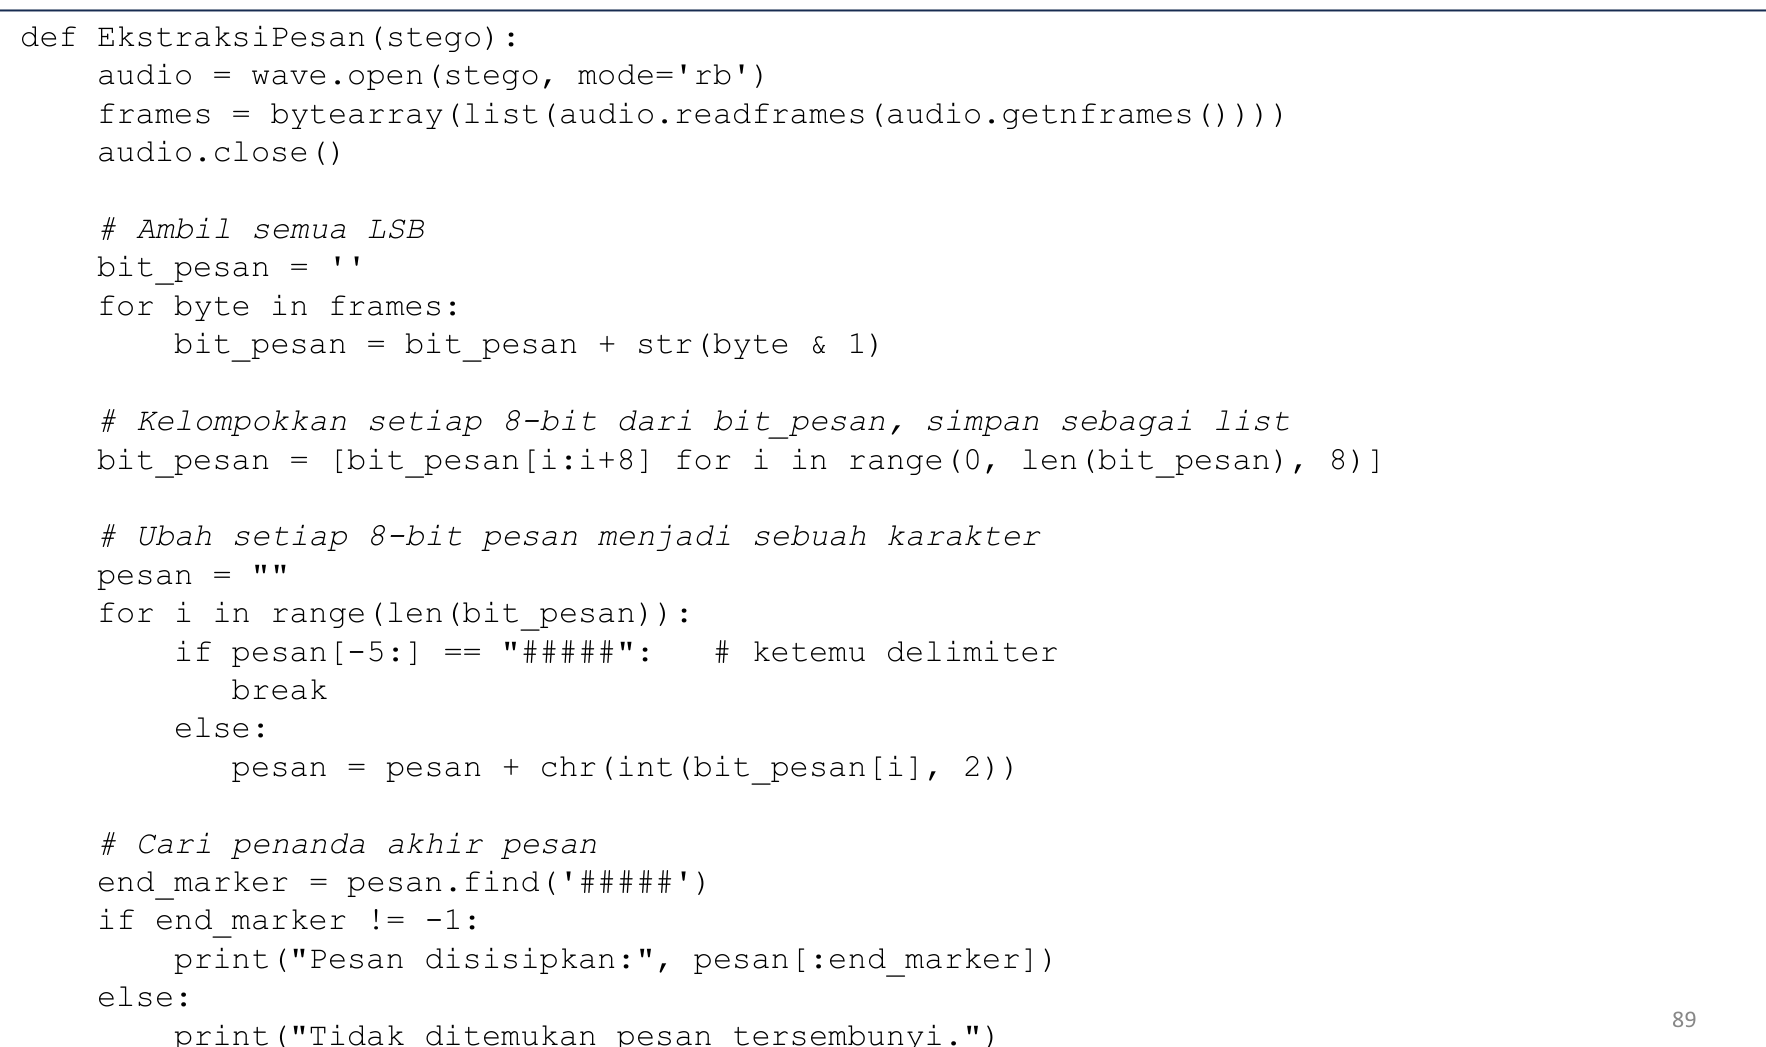
\includegraphics[width=193.20mm,height=288.09mm]{../../images/llm/page_089_img_01.png}%
\end{textblock*}

\end{document}
